\section{Architecture}
\vspace{-.3cm}In figure~\ref{fig:ears_ctrl_toolchain} we depict the architecture
of the \textsf{EARS-CTRL} tool. In the following paragraphs we will provide a
brief description of the main components of the tool's architecture, how those
components have been implemented as well as the artifacts they exchange. The
paragraphs are numbered such that each description can be matched to the
process-related components of the tool depicted in
figure~\ref{fig:ears_ctrl_toolchain}.
Letter-labels are used in figure~\ref{fig:ears_ctrl_toolchain} to refer to data
artifacts.\vspace{-.3cm}
\begin{figure}[h!] 
   \begin{center}
     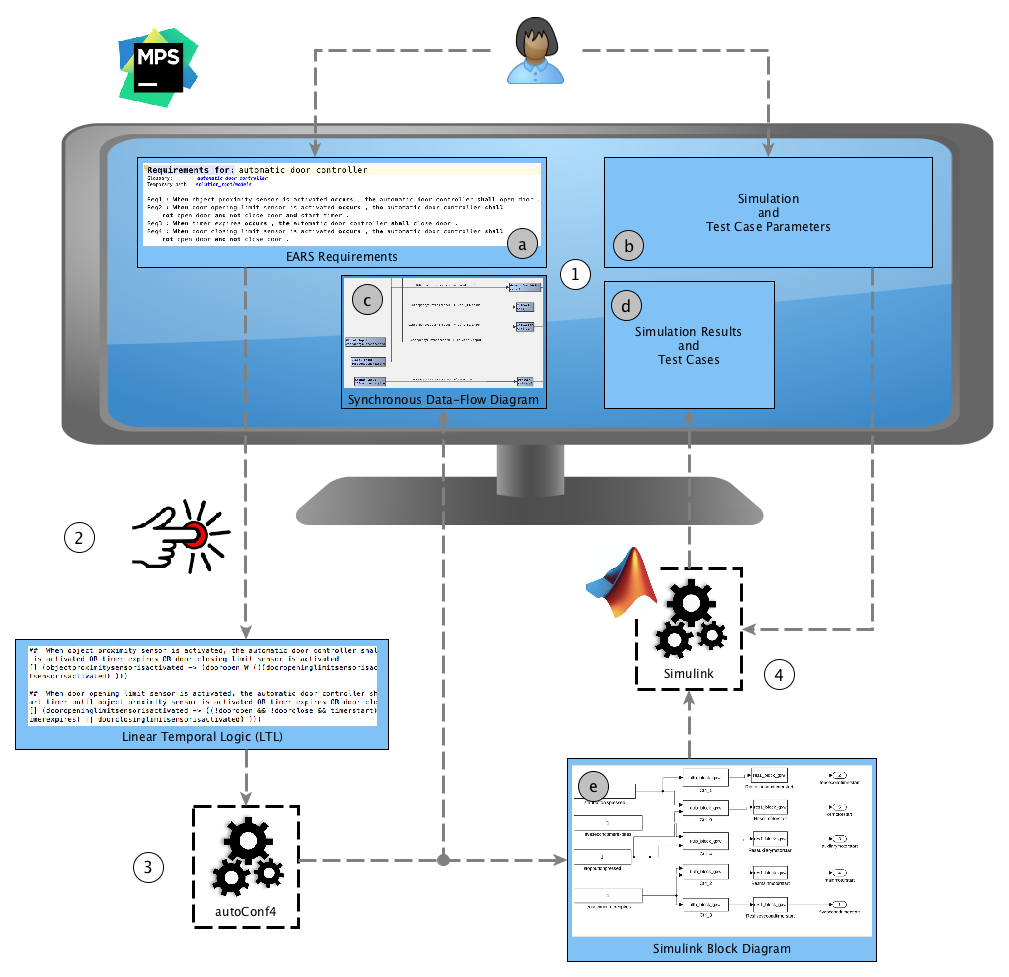
\includegraphics[width=.9\textwidth]{images/toolchain.png}
     \caption{The \textsf{EARS-CTRL} Tool Chain\levi{finish pic}}
     \label{fig:ears_ctrl_toolchain}
   \end{center}
      \vspace{-1cm}
 \end{figure}
\vspace{0cm}
\paragraph{\textbf{Editors and Control Panels}\\} 
\hspace{-.2cm}
The requirements editor, the glossary editor, the simulation and
test generation control panel and the synchonous data-flow diagram visualizer (respectively
noted (\textsf{a}), (\textsf{b}), (\textsf{c}) and (\textsf{d}) in figure~\ref{fig:ears_ctrl_toolchain}) have all been built as 
domain-specific languages (DSLs) in the Meta Programming System (MPS)
tool~\cite{mps}.
MPS is both a projectional editor and a domain-specific language workbench.
Domain-specific languages in MPS are composed of an abstract syntax, also known
as meta-model, and a concrete syntax. The concrete syntax allows displaying
and/or editing the information present in a model, as depicted for instance in
figures~\ref{fig:ears_reqs}, \ref{fig:ears_glossary} and
\ref{fig:ears_simulator}. Note that because MPS is a projectional editor, the
abstract syntax is directly edited which avoids the explicit or implicit
intermediate step where the concrete syntax is parsed.
A direct consequence of this is for example the fact that when a component's
name is updated an \textsf{EARS-CTRL} glossary, that change will immediately be
reflected in any requirements that refer to that component name. This automated
change is an off-the-shelf feature of any editor defined using MPS and an easy
way to guarantee that references between the several parts of an editor always
remain consistent.\vspace{-.2cm}
\paragraph{\textbf{From EARS to Lineal Temporal Logic}\\}
\label{sec:ears_LTL} 
\hspace{-.2cm}
Let us consider the requirement \textsf{Req1} which is part of the
specification of the sliding doors controller in figure~\ref{fig:ears_reqs}:
\begin{center}
\textbf{When} \emph{object proximity sensor is activated} \textbf{then the} \emph{automatic door controller} \textbf{shall}
\emph{open door}.
\end{center}
This requirement, taken in isolation, translates to the following LTL
 formula:
$$[] (objectproximitysensorisactivated \rightarrow dooropen)$$
which, if one takes into consideration the semantics of the $\rightarrow$
operator as ``implies'', is the expected logical meaning of \textsf{Req1}. All
EARS templates, when taken in isolation, can be directly translated into LTL and
propositional logic in such a straightforward manner. However, one translates
the whole set of requirements for the automatic door in \ref{fig:ears_reqs} into
LTL, the result for \textsf{Req1} will be as follows:
\begin{align*}
[] (object&proximitysensorisactivated \rightarrow\\
 &(dooropen\,W\,(dooropeninglimitsensorisactivated \lor timerexpires\\
 & \lor doorclosinglimitsensorisactivated )))
\end{align*}
This is due to the fact that the requirements specify behaviors that are
interwined during execution. For example, from \textsf{Req1}  in
figure~\ref{fig:ears_reqs} we know that if the \textsf{object proximity sensor}
is activated, the doors will open. We also know from \textsf{Req2} that, when
the \textsf{opening limit reached} sensor is activated, the doors will stop.
Without additional information, the \textsf{autoCode4} synthesis tool identifies
a contradition in these two requirements since, if the two sensors are activated
during the same execution, the doors will logically simultaneously open and
close. In order to avoid such contradictions it becomes necessary to establish a
temporal dependency between the behaviors specified by the requirements. To
achieve this our tool performs a static analysis of the requirements in order to
identify such dependencies and to add this information to the generated LTL
specification. This additional contextual information in the generated LTL is
clear from the second translation above:
the door will only open, \emph{until} (denoted by the ``\textbf{W}'' operator)
the door \textsf{opening limit reached} sensor is activated, \emph{or} other events
stated in door-related requirements occur.\vspace{-.2cm}
\paragraph{\textbf{Synthesizing a Controller using \textsf{autoCode4}}\\}
\hspace{-.2cm}Controller synthesis is achieved via \textsf{autoCode4}'s Java
API. The LTL specification, obtained as explained in section~\ref{sec:ears_LTL},
is passed into the synthesizer which returns a synchronous data-flow (SDF) diagram as a Java
object instance. The SDF diagram is then rebuilt as a visual model
which is an instance of the synchonous data-flow diagram visualizer DSL
(identified by label (\textsf{e}) in figure~\ref{fig:ears_reqs}). Such a visual
model provides the requirements engineer with a graphical and technical view of
the synthesized controller as a set of blocks and wires, which can be used as a
debugging artifact.\vspace{-.2cm}
\paragraph{\textbf{Simulation and Test Generation using Simulink}\\}
\hspace{-.2cm}The SDF diagram obtained from \textsf{autoCode4} consists, for
short, of a set of synchronized blocks that perform arithmetic, logical or other functions
on input signals and return the result as output signals. Note that the
controller's inputs and outputs are also themselves represented as blocks. The
fashion in which blocks are synchronized is declared by connecting those blocks'
inputs and outputs via wires. In order to simulate \textsf{EARS-CTRL}
specifications we have built a translator from such SDF diagrams onto Simulink
models. Given that the SDF formalism is very similar to the Simulink formalism,
the structural translation is  one-to-one. However, only a subset of all blocks
present in the SDF specifications that are produced by \textsf{autoCode4} is
available off-the-shelf in Simulink. As such, a number of stateful Simulink
blocks had to be built by us to mimic the semantics of some of the blocks
present in SDF specifications.

The Simulink model is generated by \textsf{EARS-CTRL} as a Mathlab simulink
script that programmatically builds the model (label (\textsf{e}) in
figure~\ref{fig:ears_reqs}). The \textsf{EARS-CTRL} IDE
communicates with Simulink via the \textsf{mathlabcontrol}\cite{mathlabcontrol}
Java API.\vspace{-.5cm}
